\chapter{Experiments and Results}
\label{cha:experimentsandresults}
%---------------------------------------------------------------------------

\section{Song Popularity}
\label{sec:songpopularity}

The analysis of song popularity provides valuable insights into the factors
that influence the success of music tracks. This problem has two approaches:
\begin{itemize}
  \item \textbf{Regression} - Spotify's popularity is a value on scale of
    0-100. This approach involves training a regression model trying to predict
    that value.
  \item \textbf{Classification} - assigning binary label to the songs(popular
    vs. unpopular) and training a classification model to predict it.
\end{itemize}

In this section the prediction of popularity was attempted using several
regression and classification models. These models were trained on different
sets of features, including Spotify metadata, lyrical attributes, and audio
features, with the aim of investigating the predictive power of those features
and their impact on popularity.

Catboost models were used as the primary predictive tool due to their
robustness and performance in handling complex relationships. 

Baseline models were also implemented to serve as a reference point:
\begin{itemize}
  \item \textit{Baseline Mean Model}: baseline model for regression that always predicts the mean.
  \item \textit{Baseline Majority Model}: baseline model for classification that always predicts the majority class.
  \item \textit{Baseline Random Model}: baseline model for classification that predicts random class.
\end{itemize}

The experiments involved both quantitative evaluatoin and SHAP analysis to
assess feature importance and interpretability of the models.

\subsection{Regression Approach}

\begin{center}
\begin{figure}[H]
  \centering
  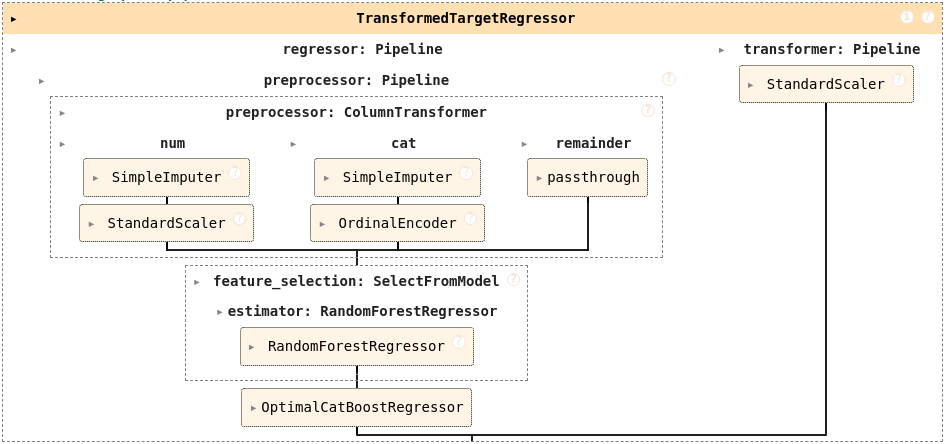
\includegraphics[width=6in]{img/reg_pipeline.png}
  \caption{Regression model pipeline. It involves preprocessing, feature
  selection and CatBoost model.}
  \label{Figure:fig_beh}
\end{figure}
\end{center}

The pipeline was fit with all available features, that includes Spotify audio
features and metadata, lyrical features and features extracted from the audio
files. The feature selection step chose the subset of most valuable features
based on the feature importance from initial Random Forest model.

% \usepackage{tabularray}
\begin{table}[H]
\centering
\caption{Results of regression of popularity.}
\begin{tblr}{
  hline{2} = {-}{},
}
 & \textbf{Model}      & \textbf{Features} & \textbf{MAE}  & \textbf{RMSE} & $R^2$         \\
 & Baseline Mean Model &                   & 13.53         & 16.90         & -0.01         \\
 & Catboost            & all               & \textbf{6.14} & \textbf{8.35} & \textbf{0.75} \\
 & Catboost            & lyrical           & 11.90         & 15.30         & 0.17          \\
 & Catboost            & spotify data      & 6.26          & 8.49          & 0.74          \\
 & Catboost            & audio             & 12.77         & 16.19         & 0.07          
\end{tblr}
\end{table}

As seen in the results table, the CatBoost model with all features achieved the
best performance, with \textbf{Mean Absolute Error(MAE) of \textbf{6.14} and
$R^2$ of 0.75}, closely followed by the model trained only on spotify metadata
and audio features. That observation shows that the spotify data offers  best
features for the task of predicting song popularity. In comparison to the
\textit{Baseline Mean Model}, the best model reduced MAE by \textbf{54.6\%} and
demonstrated a very high $R^2$.


SHAP analysis was conducted to interpret the predictions of the regression
model and asses the importance of individual features and their contribution to
song's popularity.


\begin{center}
\begin{figure}[H]
  \centering
  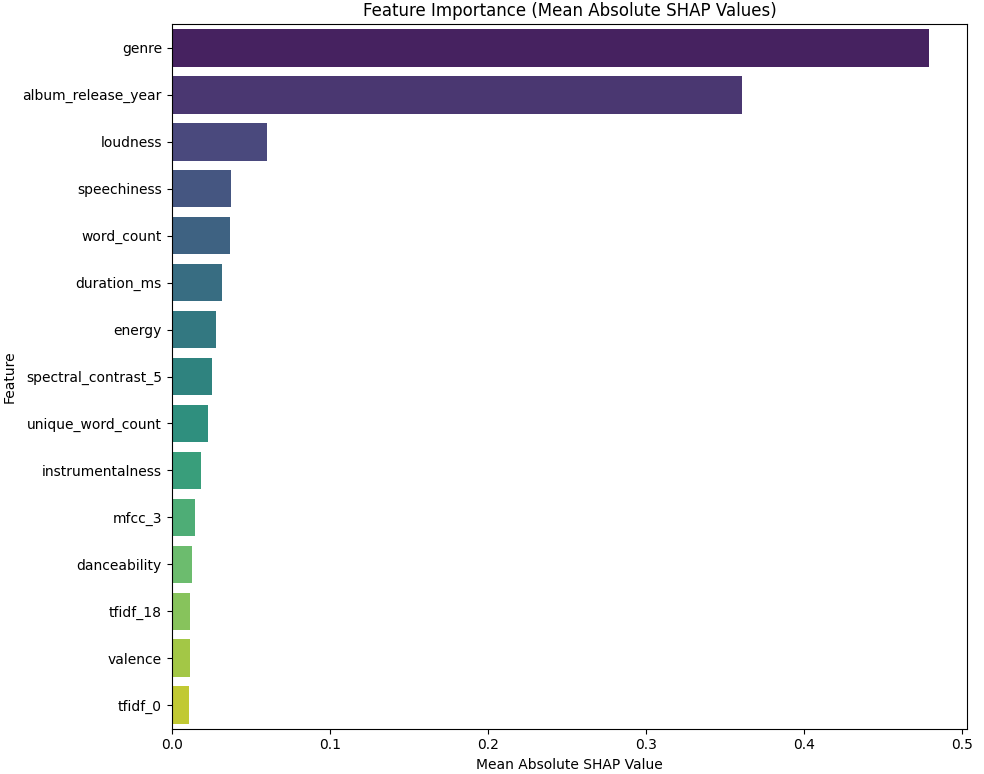
\includegraphics[width=5in]{img/feature_importance_popularity_reg.png}
  \caption{SHAP feature importance plot of the regression model for popularity.}
  \label{Figure:fig_beh}
\end{figure}
\end{center}


The mean absolute SHAP values were used to rank the overall importance of input
features. Key insights:
\begin{itemize}
  \item \textbf{Dominance of \textit{Genre} and \textit{Album Release Year}.}:
    these two features account for the majority of the predictive power in the
    model. Genre captures the musical style and release year reflects trends
    and cultural preferences over time.
  \item Spotify's audio features like \textit{loudness} and
    \textit{speachiness} showed moderate contribution to model's performance.
    Their score highlights their relevance in describing popular tracks' audio
    characteristics.
  \item Lyric-based features like \textit{word count} and \textit{unique word
    count} were significantly less impactful, however still contributed to
    model's performance to some degree.
\end{itemize}

\begin{center}
\begin{figure}[H]
  \centering
  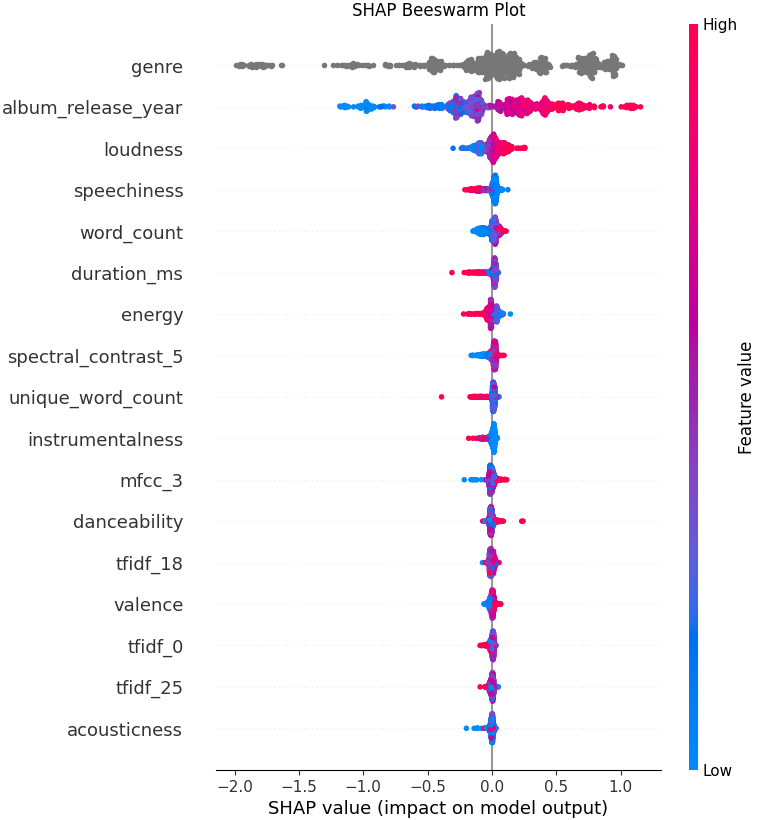
\includegraphics[width=5in]{img/beeswarm_popularity_reg.png}
  \caption{SHAP beeswarm plot of the regression model for popularity.}
  \label{Figure:fig_beh}
\end{figure}
\end{center}

\begin{itemize}
  \item Higher values of \textit{Release Year} usually result in higher
    \textit{Popularity}, which indicates that newer songs are usually more
    popular.
  \item Higher \textit{loudness} and certain levels of \textit{speechiness}
    positively correlate with higher \textit{popularity} in many cases,
    reflecting their impact on listener preferences.
\end{itemize}



\subsection{Classification Approach}

The task of predicting song popularity was reformulated as a binary
classification problem, where the target was to determine whether a song is
"popular" (1) or "not popular" (0). In order to create those labels from an
integer variable with range 0-100, the \textbf{70th perrcentile of the
popularity values was used as the threshold}. Songs with popularity greater or
equal  than this  threshold werre  labeled as popular, and the rest was labeled
as unpopular. This thresholding approach based on quantile ensures a balanced
representation of popular songs in the dataset while accounting for the
naturally skewed distribution of  popularity scores.



% \usepackage{tabularray}
\begin{table}[H]
\centering
\caption{Results of classification of popularity.}
\begin{tblr}{
  hline{2} = {-}{},
}
 & \textbf{Model}          & \textbf{Features} & \textbf{Accuracy} & \textbf{F1(w.avg.)} \\
 & Baseline Majority Model &                   & 62.90\%           & 48.57\%             \\
 & Baseline Random Model   &                   & 52.55\%           & 53.34\%             \\
 & Catboost                & all               & \textbf{84.13\%}  & \textbf{84.13\%}    \\
 & Catboost                & lyrical           & 66.75\%           & 66.25\%             \\
 & Catboost                & spotify data      & \textbf{84.41\%}  & \textbf{84.63\%}    \\
 & Catboost                & audio             & 64.55\%           & 63.73\%             
\end{tblr}
\end{table}

The classification models were evaluated using accuracy and weighted F1-score.
\textit{Baseline Majority Model} (which predicts the majority class for all samples)
achieved an accuracy of 62.90\% and an F1-score of 48.57\%. This reflects the
class imbalance introduced by the thresholding, with a higher proportion of
songs being labeled as "not popular."

The Baseline Random Model, which randomly guesses classes, performed worse than
the majority baseline in terms of accuracy (52.55\%) but achieved a slightly
higher F1-score (53.34\%) due to the randomness capturing some minority class
predictions correctly.

The CatBoost model significantly outperformed both baselines, achieving an
overall accuracy of 84.13\% and a weighted F1-score of 84.13\% trained on all
features.

CatBoost trained on Spotify data managed to slightly outperform the model
trained on all features, further reinforcing the observation that Spotify audio
features and metadata are the strongest predictors of popularity.

The model using only lyrical features showed relatively lower performance, with
an accuracy of 66.75\% and an F1-score of 66.25\%. This indicates that while
lyrics contribute to song popularity, they are far less predictive than other
feature sets.

The performance of the model trained on features extracted from audio files was
similar to the lyrical one, demonstrating that isolated audio features are not
suffficient to fully predict popularity.


SHAP analysis was conducted to understand the feature dependencies and
importance for the classification task. As expected, the results were
consistent with the regression analysis of popularity. Key features such as
\textit{genre}, \textit{album release year}, \textit{danceability}, and \textit{loudness} emerged as the most
significant predictors, mirroring their importance in the regression task. This
consistency underscores the robustness of these features in modeling song
popularity across different approaches (regression and classification).

\begin{center}
\begin{figure}[H]
  \centering
  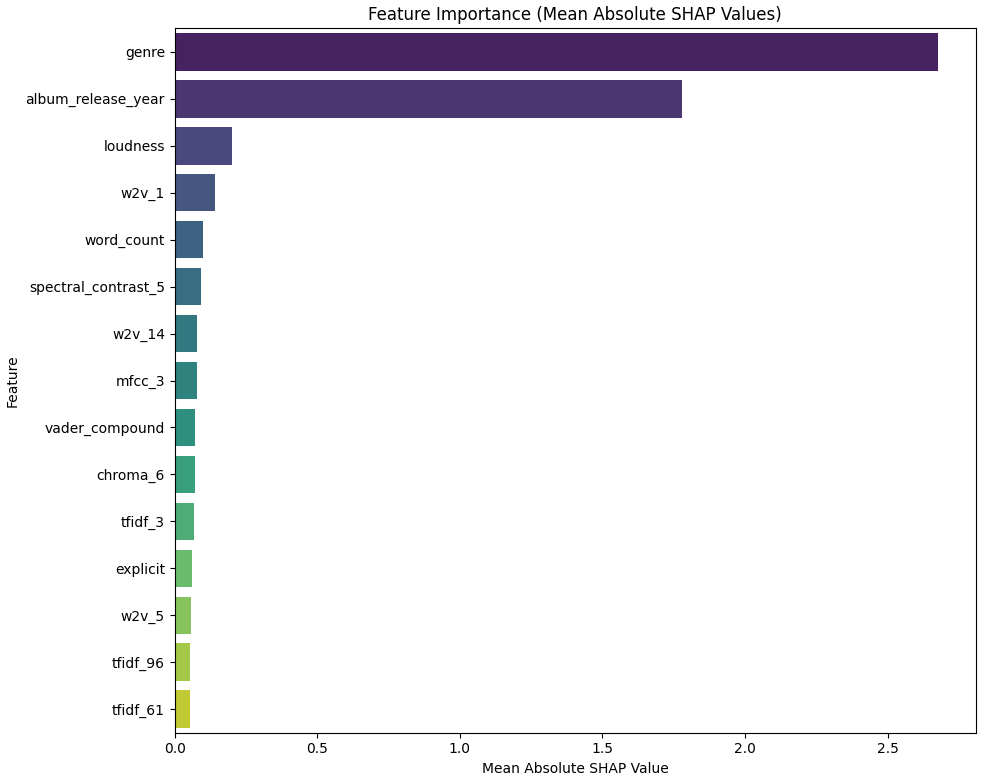
\includegraphics[width=5in]{img/feature_importance_popularity_clf.png}
  \caption{SHAP feature importance plot of the classification model for popularity.}
  \label{Figure:fig_beh}
\end{figure}
\end{center}

\begin{center}
\begin{figure}[H]
  \centering
  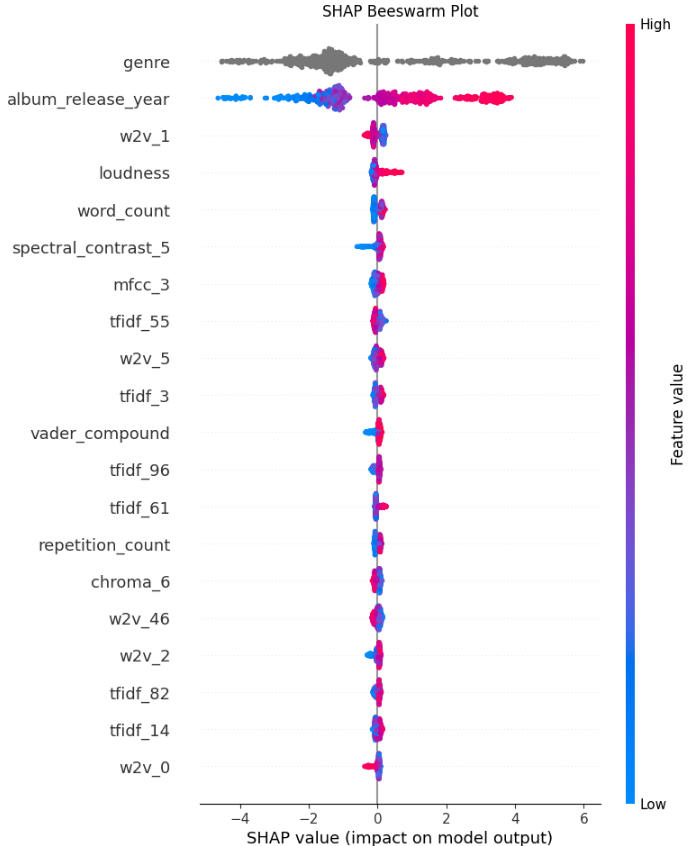
\includegraphics[width=5in]{img/beeswarm_popularity_clf.png}
  \caption{SHAP beeswarm plot of the classification model for popularity.}
  \label{Figure:fig_beh}
\end{figure}
\end{center}



The SHAP analysis for the classification model highlights similar dependencies
to the regression model. Key features like \textit{genre} and
\textit{album release year} remain the most important, emphasizing their role
in shaping song popularity. 

Several differences can be observed between feature importance in the
regression and classification model, notably:
\begin{itemize}
  \item Lyrics embeddings(TF-IDF and Word2Vec) seemed to play a bigger role in
    the classification model.
  \item Classification model seemed to pay much less attention to Spotify audio
    features, like \textit{danceability}, \textit{energy} and
    \textit{speechiness}.
  \item Unlike in regression, in classification a sentiment metric,
    \textit{VADER compound} contributed to the prediction of popularity. More
    popular songs tend to have more positive lyrics.
\end{itemize}

\section{Explicitness}
\label{sec:explicitness}

The task of predicting whether a song contains explicit content was approached
as a classification problem. The performance of the CatBoost model was compared
against baseline on different feature subsets. One of the key challenges of
this problem was significant class imbalance present in the dataset;
approximately 85\% of the songs did not contain explicit content.

Significant class imbalance can lead to models favoring the majority class,
potentially resulting in  high accuracy but poor performance on the minority
class. To address this problem, CatBoost's class weights parameter was used.
This parameter allowed the model to penalize misclassifications of the minority
class more heavily, therefore improving its ability to recognize explicit
content.

% \usepackage{tabularray}
\begin{table}[H]
\centering
\caption{Results of classification of explicitness.}
\begin{tblr}{
  hline{2} = {-}{},
}
 & \textbf{Model}          & \textbf{Features} & \textbf{Accuracy} & \textbf{F1 weighted average} \\
 & Baseline Majority Model &                   & 84.00\%           & 76.69\%                      \\
 & Baseline Random Model   &                   & 50.06\%           & 56.57\%                      \\
 & Catboost                & all               & \textbf{92.68\%}  & \textbf{92.72\%}             \\
 & Catboost                & lyrical           & \textbf{92.55\%}  & \textbf{92.41\%}             \\
 & Catboost                & spotify data      & 85.93\%           & 86.41\%                      \\
 & Catboost                & audio             & 84.13\%           & 83.03\%                      
\end{tblr}
\end{table}

The table presents the results of the models in terms of accurracy and weighted
F1 score. The \textit{Baseline Majority Model} achieved accuracy of 84\% and
significantly lower F1 weighted average of 76.69\%, which reflects its inability
to handle class balance effectively. The \textit{Baseline Random Model}
performed very poorly, with an accuracy of 50.06\% and F1 weighted average of
56.57\%.

In contrast, the CatBoost model outperformed both baselines achieving accuracy
of \textbf{92.68\%} and weighted average score of \textbf{92.72\%} when trained
on all features. Interestingly, the model trained only using lyrical features
performed nearly as well, indicating that explicitness can larrgely be
predicted based on lyrrical content. Models that relied on Spotify metadata and
features extracted from audio files had lower performance, achieving accurracy
close to \textit{Baseline Majority Model}, but with higher F1 scores. This
observation emphasizes the centrality of lyrical information in prediction of
explicit content.


\begin{center}
\begin{figure}[H]
  \centering
  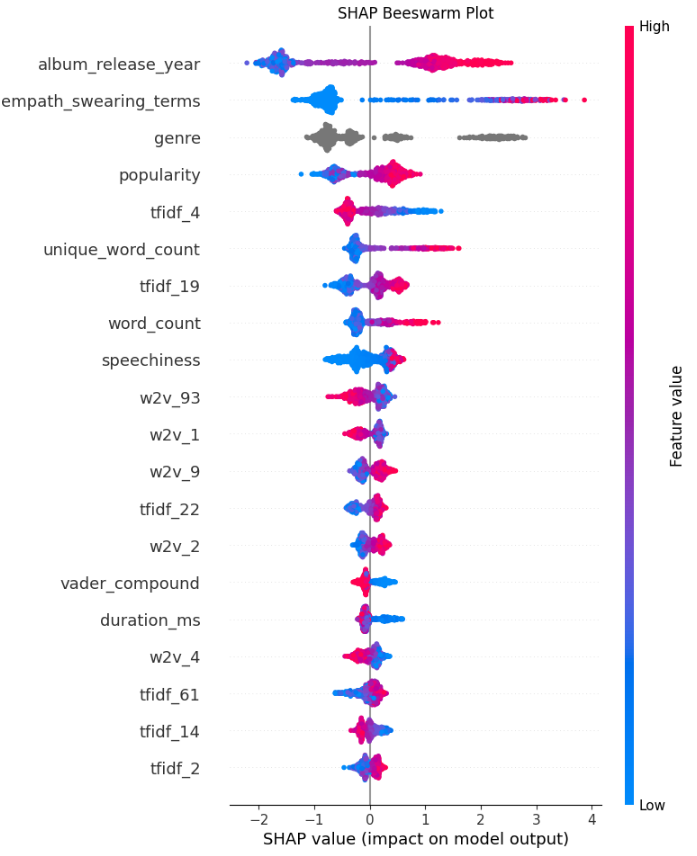
\includegraphics[width=5in]{img/beeswarm_explicitness.png}
  \caption{SHAP beeswarm plot of the classification model for explicitness.}
  \label{Figure:fig_beh}
\end{figure}
\end{center}

\begin{center}
\begin{figure}[H]
  \centering
  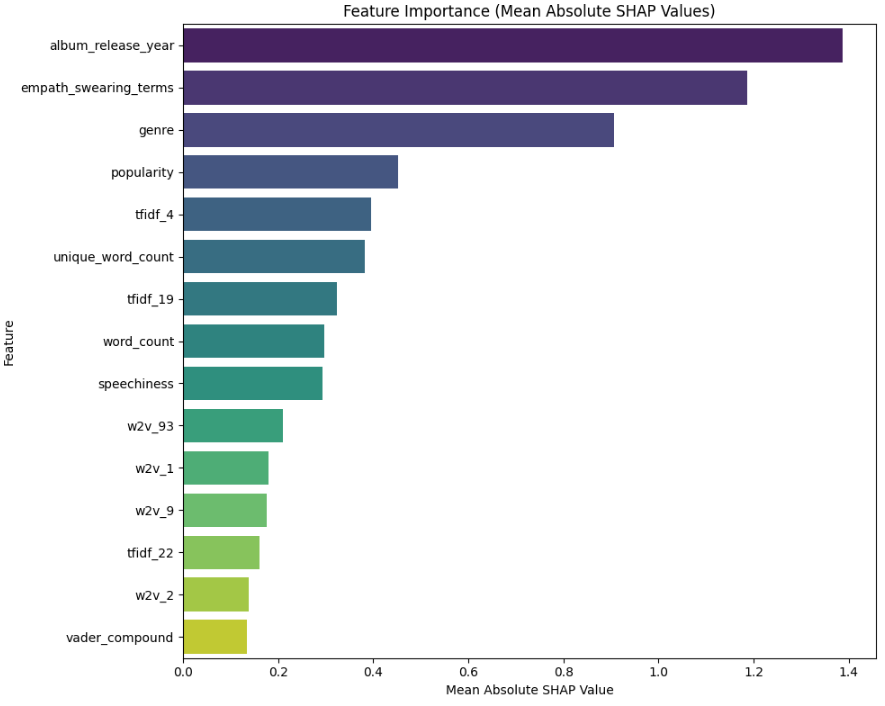
\includegraphics[width=5in]{img/feature_importance_explicitness.png}
  \caption{SHAP beeswarm plot of the classification model for explicitness.}
  \label{Figure:fig_beh}
\end{figure}
\end{center}


Key features for this task turned out to be:
\begin{itemize}
  \item \textbf{Album Release Year}: this feature had  highest feature
    importance, reflecting temporal trends in explicit content. Newer songs are
    statistically more likely to contain explicit language, reflecting changing
    societal norms and artistic expressions over time.
  \item \textbf{Empath Swearing Terms}: As expected, the presence of swearing
    terms was a strong indicator of explicitness.
  \item \textbf{Genre} was the third most important feature, showing that
    certain genres  are more likely to contain explicit content than others.
  \item \textbf{TF-IDF}: several vectors created using TF-IDF and later reduced
    via PCA significantly contributed to the model's predictions. Similar to
    the Empath feature, TF-IDF likely captured swear words and related patterns
    in the lyrics, reinforcing its importance.
  \item \textbf{Speechiness}: songs with higher values of
    speechiness—indicating a greater presence of spoken-word elements—were more
    likely to be labeled as explicit.
\end{itemize}
